\documentclass[11pt,a4paper]{article}

\usepackage[utf8]{inputenc}
\usepackage[T1]{fontenc}
\usepackage[spanish]{babel}
\usepackage[margin=2.5cm]{geometry}
\usepackage{graphicx,tabularx,longtable,array,fancyhdr}
\usepackage[table]{xcolor}
\usepackage[hidelinks]{hyperref}
\usepackage[backend=biber,style=ieee]{biblatex}
\addbibresource{referencias.bib}

\setlength{\headheight}{14pt}
\setlength{\parindent}{0pt}
\setlength{\parskip}{6pt}
\setlength{\emergencystretch}{1.5em}
\renewcommand{\arraystretch}{1.23}

\pagestyle{fancy}
\fancyhf{}
\fancyhead[L]{\small UTEQ · Ingeniería de Requerimientos}
\fancyhead[R]{\small TA-IND-01}
\fancyfoot[L]{\small Angelo Espinoza}
\fancyfoot[R]{\small Página \thepage}

\begin{document}

\begin{center}
    {\large\textbf{UNIVERSIDAD TÉCNICA ESTATAL DE QUEVEDO}}

    Facultad de Ciencias de la Computación\\
    Carrera de Software

    \vspace{0.6cm}
    {\LARGE\textbf{IEEE 29148 y tipos de requisitos}}\\[4pt]
    {\large Análisis de YouTube Web}

    \vspace{0.2cm}
    {\large TA-IND-01}\\
    Actividad sumativa individual
\end{center}

\vspace{0.4cm}

\section{Datos informativos}

\begin{tabularx}{\textwidth}{|l|X|}
\hline
\rowcolor{gray!15}
\textbf{Campo} & \textbf{Detalle} \\ \hline
Estudiante & Angelo Maximiliano Espinoza Pivaque \\ \hline
Asignatura & Ingeniería de Requerimientos (ISR-401) \\ \hline
Nivel y paralelo & Cuarto nivel, paralelo A \\ \hline
Docente & Gleiston Cicerón Guerrero Ulloa, PhD \\ \hline
Caso & YouTube Web \\ \hline
Fecha de entrega & 11 de noviembre de 2026 \\ \hline
\end{tabularx}

\section{Descripción y alcance}

YouTube Web permite buscar, ver y organizar videos desde el navegador.
El análisis se centra en el espectador que usa la plataforma en una
computadora. Se estudian tres recorridos: buscar un tema, reproducir
un video de los resultados y consultar las listas de reproducción.
Como ejemplo se utiliza la búsqueda de contenido sobre jerarquía de memoria.

\section{Resumen analítico de la norma}

Un requisito transforma una necesidad en una condición que se puede discutir
y comprobar. La cláusula 5.2.4 de ISO/IEC/IEEE 29148:2018 orienta la
redacción del enunciado \cite[cl. 5.2.4]{ieee29148}. Para el caso de
YouTube Web, una forma práctica de aplicarla es identificar el sujeto, el
comportamiento esperado y las condiciones pertinentes. Por ejemplo, la
necesidad de encontrar material para estudiar se puede expresar así:
«Cuando el espectador envíe una consulta de texto, YouTube Web deberá
mostrar la página de resultados de esa consulta». La condición distingue
la búsqueda ejecutada del simple hecho de escribir en la barra.

\subsection{Características de un requisito individual}

La cláusula 5.2.5 propone nueve características para revisar cada
enunciado \cite[cl. 5.2.5]{ieee29148}. Aplicadas al caso, permiten
examinar lo siguiente:

\begin{enumerate}
\item \textbf{Necesario.} Debe responder a una necesidad del espectador.
Pausar un tutorial le permite detenerse para tomar apuntes.

\item \textbf{Apropiado.} El detalle debe corresponder al nivel del análisis.
Para pedir que aparezcan resultados basta describir lo observable en el navegador.

\item \textbf{No ambiguo.} Debe admitir una interpretación clara.
«Tiempo transcurrido» se refiere al punto actual de reproducción.

\item \textbf{Completo.} Debe incluir la información necesaria para entender
qué se espera. Si el requisito trata de una lista personal, conviene indicar
que la sesión está iniciada.

\item \textbf{Singular.} Debe expresar una obligación principal. Pausar
un video y guardarlo en una lista se comprueban por separado.

\item \textbf{Factible.} Debe poder realizarse dentro de las condiciones y
recursos disponibles. Un tiempo de respuesta se plantea para un equipo y
una red concretos.

\item \textbf{Verificable.} Debe permitir reunir evidencia de cumplimiento.
Para comprobar la pausa se observa si el contador deja de avanzar.

\item \textbf{Correcto.} Debe reflejar la necesidad real. Si el espectador
quiere volver a un video, el criterio debe comprobar que puede encontrarlo
en la lista elegida.

\item \textbf{Conforme.} Debe seguir el formato acordado. En esta tarea,
cada requisito tiene identificador, tipo y criterio de aceptación.
\end{enumerate}

Estas características se complementan. Una frase puede ser clara y aun
así estar incompleta si omite una condición decisiva. «Mostrar mis listas»
es comprensible, pero todavía necesita indicar a qué cuenta pertenecen
las listas que se espera ver. Revisar esa condición antes de redactar la
prueba evita que dos personas evalúen situaciones diferentes.

\subsection{Características del conjunto de requisitos}

La cláusula 5.2.6 permite revisar la especificación como un todo
\cite[cl. 5.2.6]{ieee29148}. Para que el conjunto sea \textbf{completo},
debe cubrir el alcance acordado: búsqueda, reproducción y listas. La
\textbf{consistencia} exige que los enunciados usen los términos de forma
estable y que sus condiciones sean compatibles. Por ejemplo, un requisito
puede permitir buscar sin iniciar sesión y otro exigir una sesión para
guardar en una lista personal. Precisar la condición de cada uno permite
interpretarlos en conjunto.

La \textbf{factibilidad} se evalúa también para todos los requisitos
juntos: las metas de rendimiento y facilidad de uso deben poder
comprobarse con un entorno y un método definidos. El conjunto debe ser
\textbf{comprensible}, de modo que el lector entienda qué cubre y cómo se
relacionan sus partes. Por último, debe \textbf{poder validarse} frente a
la necesidad original. Un recorrido de prueba en el que el espectador
busca un tutorial, abre el resultado y lo guarda en una lista permite
revisar si los requisitos, vistos en conjunto, respaldan su objetivo.

\subsection{Lenguaje que conviene evitar}

La cláusula 5.2.7 advierte sobre expresiones que hacen difícil interpretar
o comprobar un requisito \cite[cl. 5.2.7]{ieee29148}. En este ejercicio,
«rápido» o «fácil» requieren una medida. «El mejor reproductor» introduce
un superlativo sin criterio. «Mejor que antes» deja sin identificar la
referencia de comparación, mientras que «si es posible» permite omitir
el comportamiento sin especificar en qué condiciones. Los pronombres
como «esto» pueden perder su referente y expresiones abiertas como
«entre otros» dejan indefinido qué elementos se evaluarán. También
conviene revisar absolutos como «siempre», conectores como «y/o» y
referencias incompletas cuya versión o alcance no se pueda identificar.

Una corrección concreta es reemplazar «la búsqueda debe ser rápida»
por un tiempo máximo para una consulta y un entorno definidos. El tiempo
se mide desde el envío de la consulta hasta que aparece el primer
resultado. El valor elegido es un objetivo del ejercicio, y la prueba
debe registrar el resultado real. Esta distinción permite comparar lo
que el requisito pide con lo que se observa en la plataforma.

\section{Glosario}

\section{Requisitos y criterios de aceptación}

Se distinguen cinco tipos: funcional, interfaz, restricción de diseño,
rendimiento y usabilidad. Rendimiento y usabilidad agrupan los cinco
requisitos de calidad, clasificados según ISO/IEC 25010:2023
\cite{iso25010}. Los umbrales y restricciones son propuestas del ejercicio.
Para las pruebas de tiempo se propone Chrome de escritorio, ventana de
1366 por 768 píxeles y conexión estable de al menos 20 Mb/s de descarga.
En las pruebas del reproductor se usa un video público disponible, una vez
que se pueda reproducir el contenido.

\begingroup
\small
\setlength{\tabcolsep}{4pt}
\renewcommand{\arraystretch}{1.25}

\begin{longtable}{|p{.085\textwidth}|p{\dimexpr.915\textwidth-4\tabcolsep-3\arrayrulewidth\relax}|}

\hline
\rowcolor{gray!15}
\textbf{Código} & \textbf{Clasificación y criterio de aceptación} \\ \hline
\endfirsthead

\hline
\rowcolor{gray!15}
\textbf{Código} & \textbf{Clasificación y criterio de aceptación} \\ \hline
\endhead

\textbf{RF-01} &
\textbf{Enunciado:} YouTube Web deberá mostrar una página de resultados al enviar una consulta de texto.\newline
\textbf{Tipo:} Funcional.\newline
\textbf{Criterio de aceptación:} Buscar «jerarquía de memoria» y verificar que aparece una página con resultados de esa consulta.
\\ \hline

\textbf{RF-02} &
\textbf{Enunciado:} YouTube Web deberá abrir el reproductor del video seleccionado desde los resultados.\newline
\textbf{Tipo:} Funcional.\newline
\textbf{Criterio de aceptación:} Elegir un resultado y comprobar que el título abierto coincide con el seleccionado.
\\ \hline

\textbf{RF-03} &
\textbf{Enunciado:} YouTube Web deberá pausar el video cuando el espectador pulse el control de pausa durante la reproducción.\newline
\textbf{Tipo:} Funcional.\newline
\textbf{Criterio de aceptación:} Pulsar pausa y observar que el tiempo deja de avanzar.
\\ \hline

\textbf{RF-04} &
\textbf{Enunciado:} YouTube Web deberá mostrar las listas de reproducción disponibles para la cuenta con sesión iniciada.\newline
\textbf{Tipo:} Funcional.\newline
\textbf{Criterio de aceptación:} Abrir Playlists con una cuenta que tenga una lista y verificar que esta aparece.
\\ \hline

\textbf{RI-01} &
\textbf{Enunciado:} YouTube Web deberá mostrar el tiempo transcurrido y la duración total en los controles de un video pregrabado.\newline
\textbf{Tipo:} Interfaz.\newline
\textbf{Criterio de aceptación:} Hacer visibles los controles y comprobar que se muestran ambos tiempos.
\\ \hline

\textbf{RI-02} &
\textbf{Enunciado:} YouTube Web deberá mostrar el nombre y el conteo de videos en cada tarjeta de lista personal.\newline
\textbf{Tipo:} Interfaz.\newline
\textbf{Criterio de aceptación:} Abrir Playlists y cotejar esos dos datos con el contenido de una lista de prueba.
\\ \hline

\textbf{RF-05} &
\textbf{Enunciado:} YouTube Web deberá reanudar un video pausado al activar el control de reproducción.\newline
\textbf{Tipo:} Funcional.\newline
\textbf{Criterio de aceptación:} Pausar un video, activar reproducción y comprobar que el contador vuelve a avanzar.
\\ \hline

\textbf{RF-06} &
\textbf{Enunciado:} YouTube Web deberá abrir la vista de una lista al seleccionar su tarjeta.\newline
\textbf{Tipo:} Funcional.\newline
\textbf{Criterio de aceptación:} Seleccionar una lista que contenga un video y comprobar que se muestra ese video en la vista abierta.
\\ \hline

\textbf{RD-01} &
\textbf{Enunciado:} El recorrido de búsqueda y reproducción deberá poder completarse desde Chrome de escritorio sin instalar extensiones.\newline
\textbf{Tipo:} Restricción de diseño.\newline
\textbf{Criterio de aceptación:} Usar un perfil con extensiones deshabilitadas, buscar un video público y reproducirlo.
\\ \hline

\textbf{RD-02} &
\textbf{Enunciado:} El acceso a listas personales deberá requerir una sesión de usuario activa.\newline
\textbf{Tipo:} Restricción de diseño.\newline
\textbf{Criterio de aceptación:} Con la sesión cerrada, abrir la URL de una lista privada propia y comprobar que su contenido no se muestra.
\\ \hline

\textbf{RC-01} &
\textbf{Enunciado:} YouTube Web deberá mostrar el primer resultado en hasta 3 segundos al enviar la consulta «jerarquía de memoria».\newline
\textbf{Tipo:} Rendimiento.\newline
\textbf{ISO/IEC 25010:2023:} Eficiencia de desempeño / comportamiento temporal.\newline
\textbf{Criterio de aceptación:} Medir del envío al primer resultado visible. Umbral: hasta 3 s en al menos 4 de 5 intentos.
\\ \hline

\textbf{RC-02} &
\textbf{Enunciado:} Con un video ya cargado y en reproducción, el control de pausa deberá detener el avance en hasta 500 ms.\newline
\textbf{Tipo:} Rendimiento.\newline
\textbf{ISO/IEC 25010:2023:} Eficiencia de desempeño / comportamiento temporal.\newline
\textbf{Criterio de aceptación:} Medir en una grabación de pantalla desde la pulsación hasta la detención visible. Umbral: hasta 500 ms en al menos 4 de 5 intentos.
\\ \hline

\textbf{RC-03} &
\textbf{Enunciado:} YouTube Web deberá permitir pausar y reanudar con la barra espaciadora cuando el reproductor tenga el foco.\newline
\textbf{Tipo:} Usabilidad.\newline
\textbf{ISO/IEC 25010:2023:} Capacidad de interacción / operabilidad.\newline
\textbf{Criterio de aceptación:} Contar pulsaciones en cinco ciclos. Umbral: una pulsación por acción en los cinco ciclos.
\\ \hline

\textbf{RC-04} &
\textbf{Enunciado:} YouTube Web deberá permitir silenciar un video mediante una activación del control de sonido visible.\newline
\textbf{Tipo:} Usabilidad.\newline
\textbf{ISO/IEC 25010:2023:} Capacidad de interacción / operabilidad.\newline
\textbf{Criterio de aceptación:} Comenzar con audio audible y contar activaciones. Umbral: una por intento en cinco intentos.
\\ \hline

\textbf{RC-05} &
\textbf{Enunciado:} YouTube Web deberá permitir activar subtítulos en español en hasta dos activaciones desde los controles visibles de un video que ya tenga esa pista seleccionada.\newline
\textbf{Tipo:} Usabilidad.\newline
\textbf{ISO/IEC 25010:2023:} Capacidad de interacción / asistencia al usuario.\newline
\textbf{Criterio de aceptación:} Con subtítulos desactivados, contar activaciones hasta que aparezca el primer texto hablado. Umbral: hasta dos en cinco intentos.
\\ \hline

\end{longtable}
\endgroup

\section{Autoevaluación}

\section{Reflexión}

\section{Evidencias del sistema}

\begin{figure}[htbp]
    \centering
    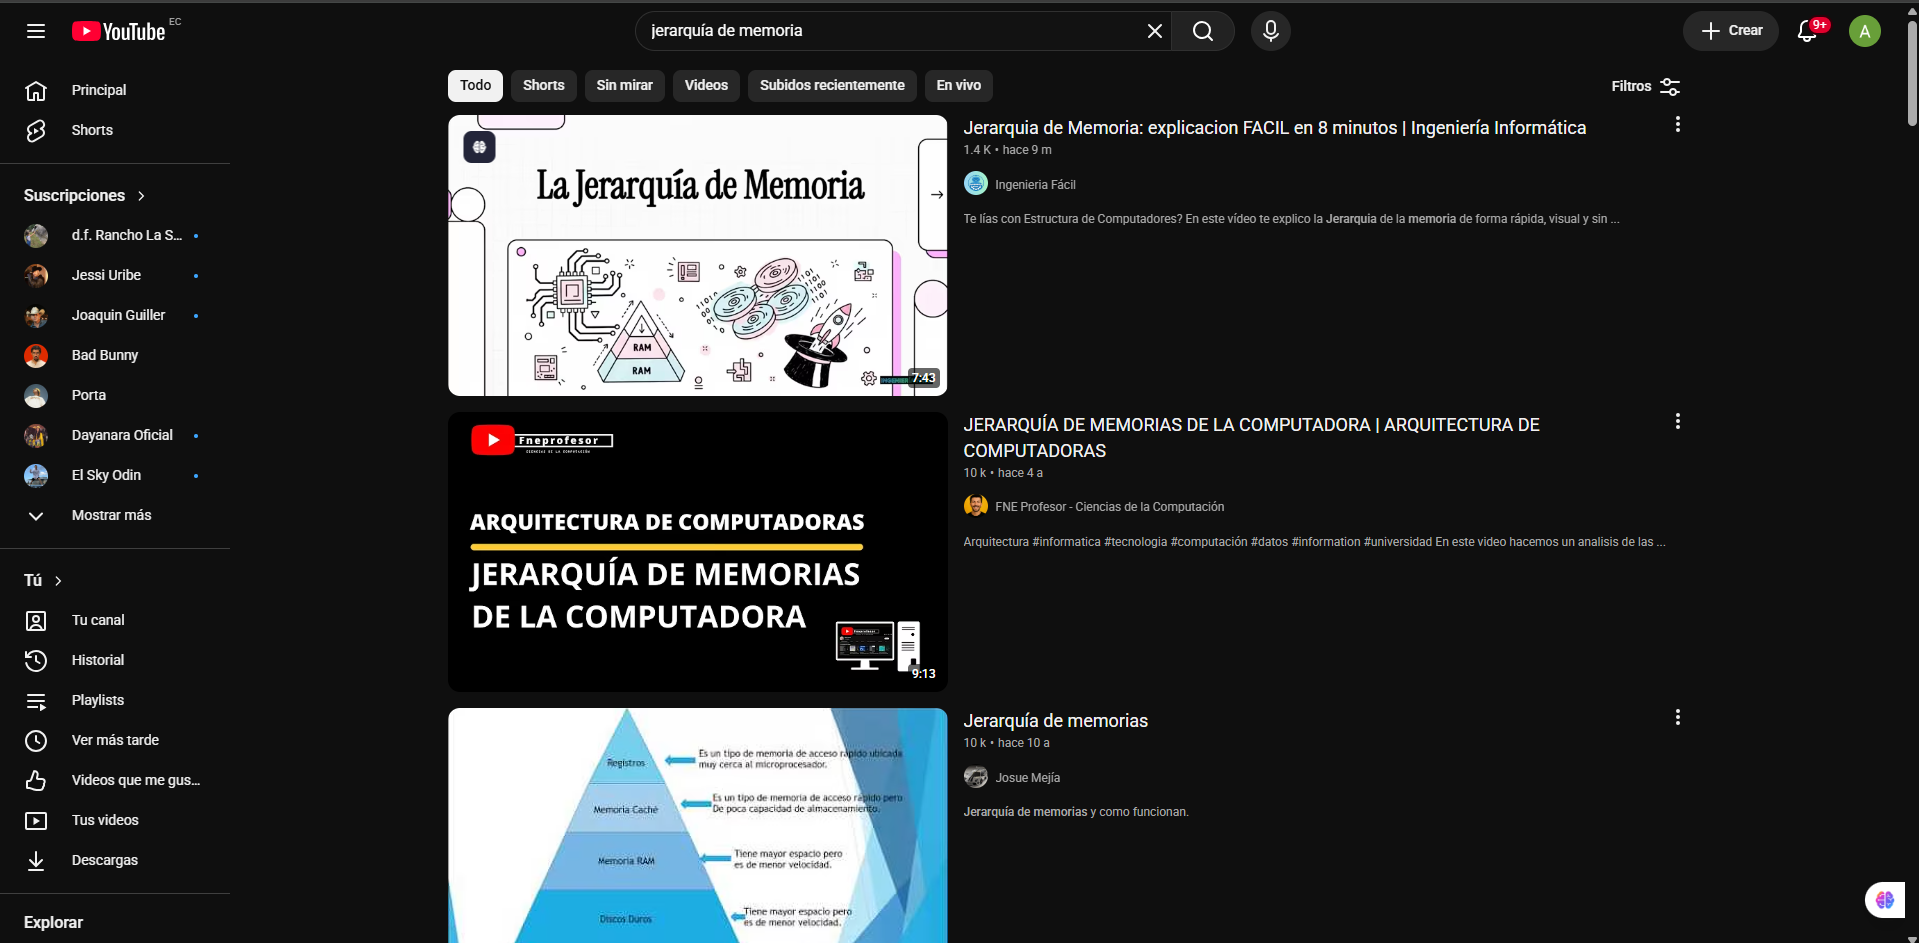
\includegraphics[width=.90\linewidth]{figuras/busqueda.png}
    \caption{Resultados de la búsqueda «jerarquía de memoria».}
\end{figure}

\begin{figure}[htbp]
    \centering
    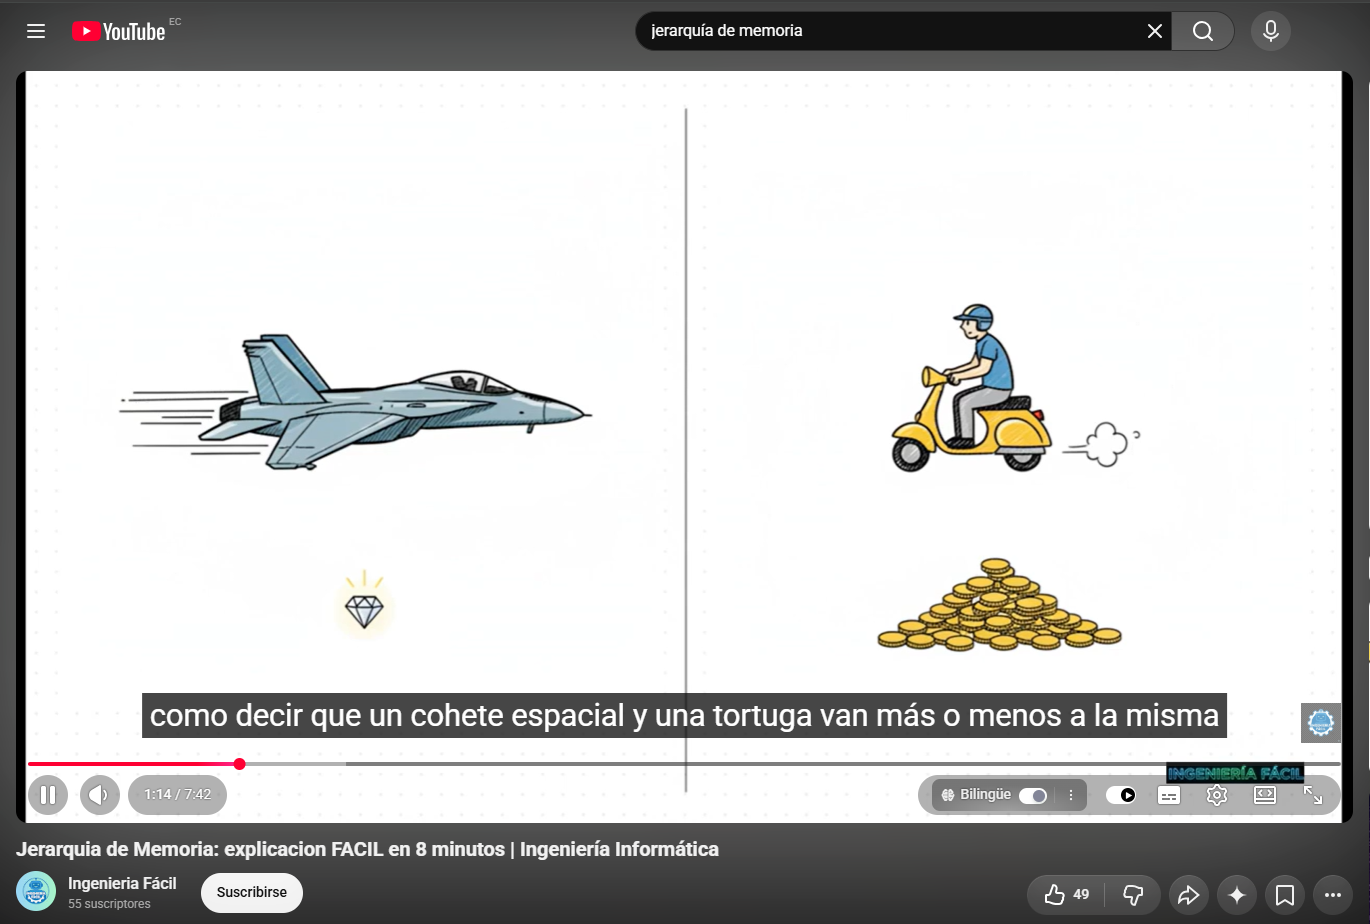
\includegraphics[width=.80\linewidth]{figuras/reproduccion.png}
    \caption{Reproductor con controles, tiempos y subtítulos visibles.}
\end{figure}

\begin{figure}[htbp]
    \centering
    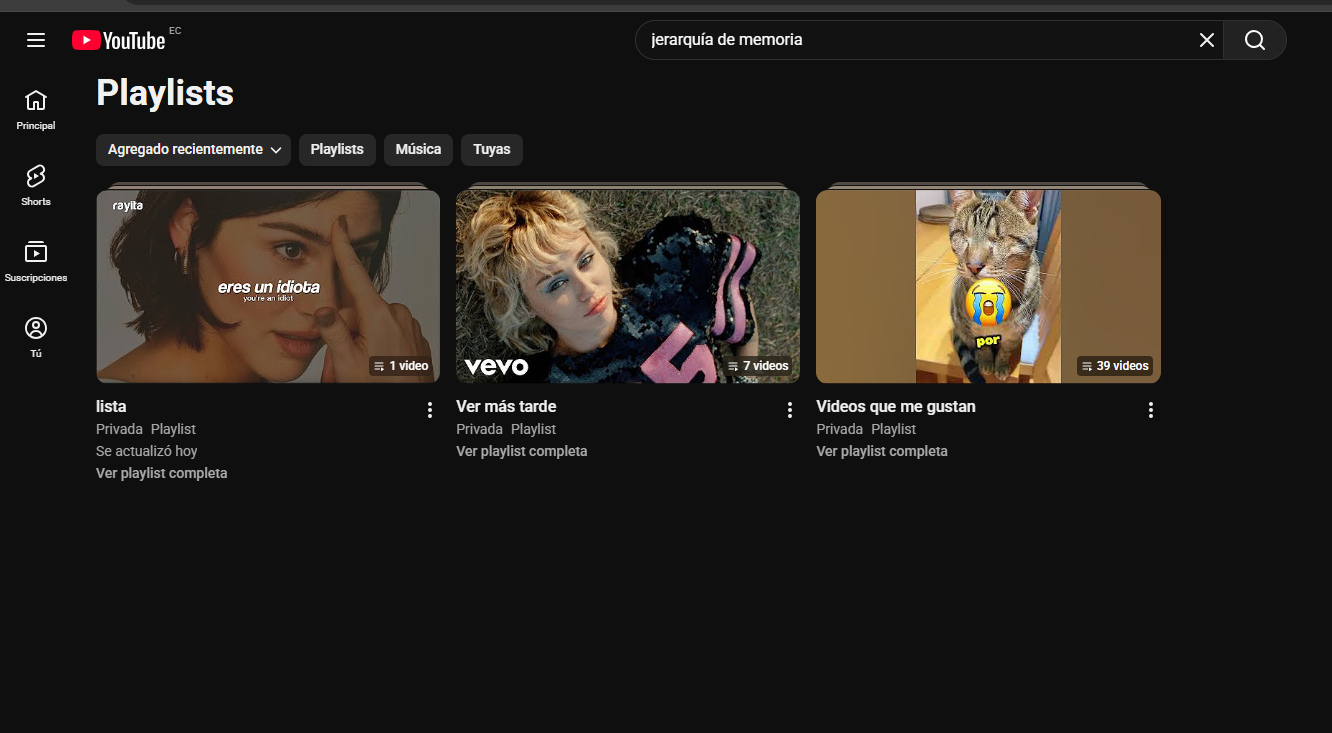
\includegraphics[width=.90\linewidth]{figuras/listas.png}
    \caption{Vista de listas con sus nombres y conteos de videos.}
\end{figure}

\clearpage
\printbibliography[title={Referencias}]

\end{document}